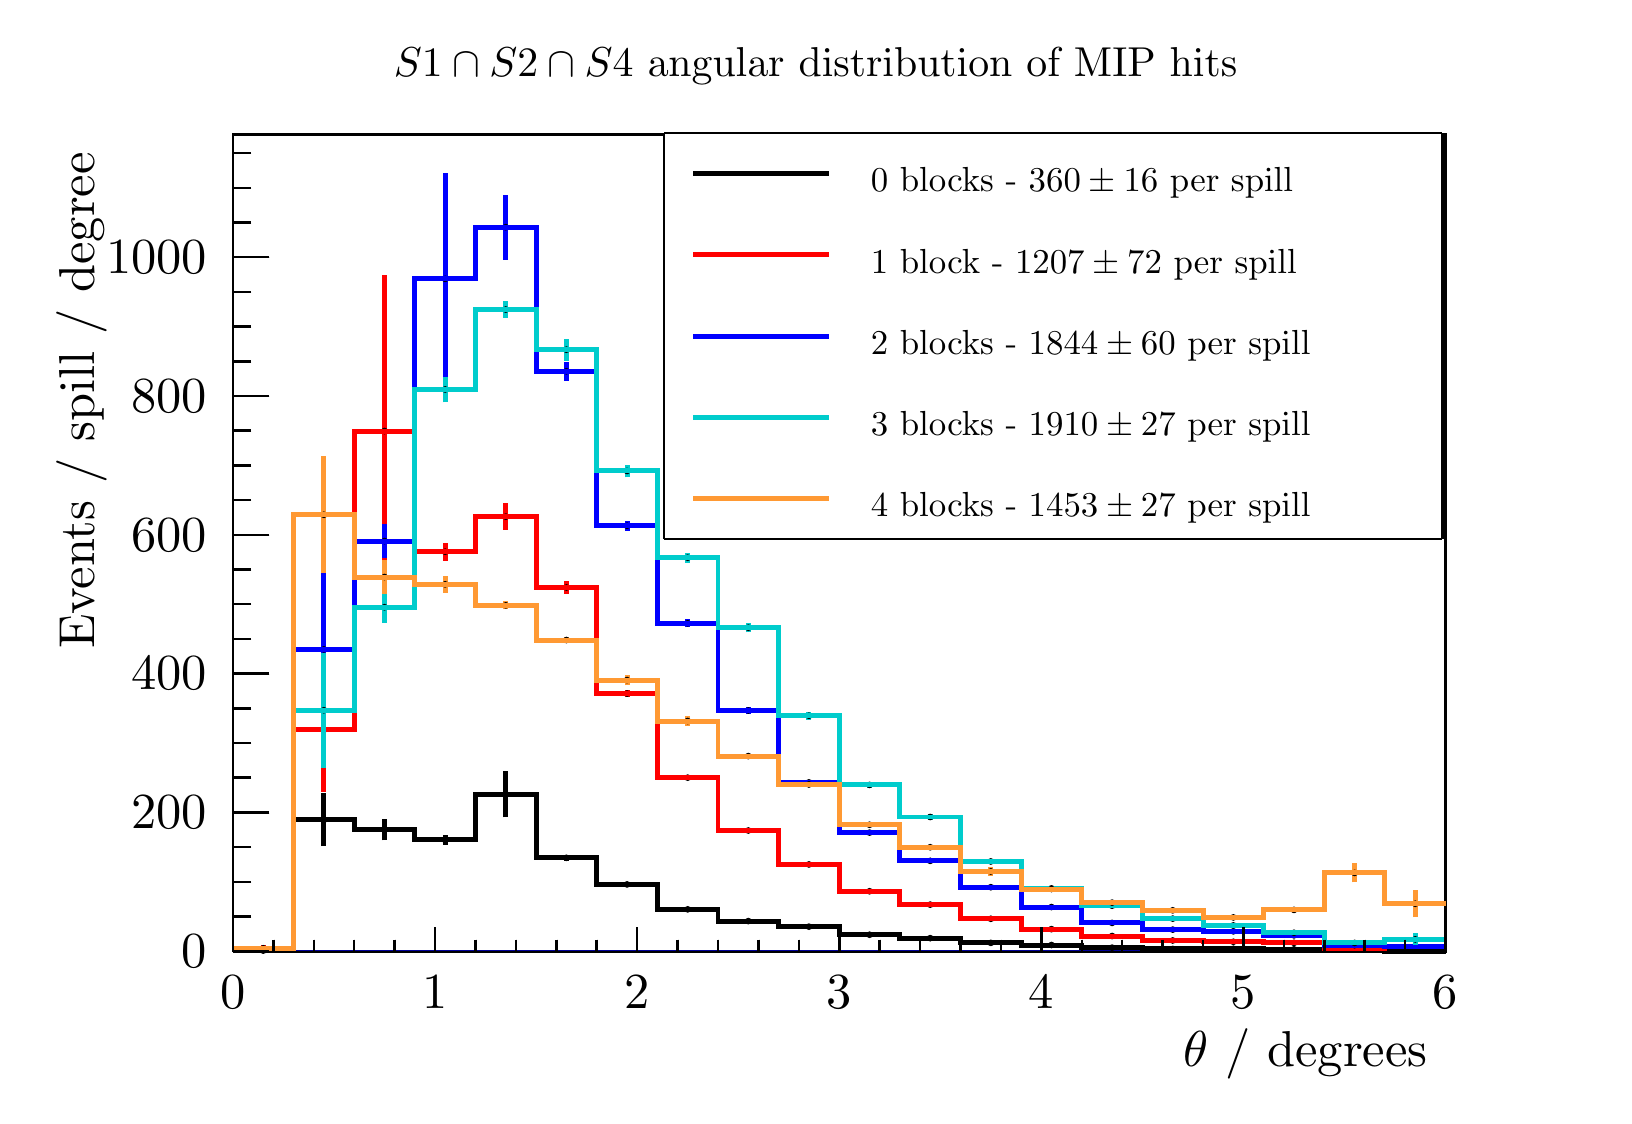
\begin{tikzpicture}
\pgfdeclareplotmark{cross} {
\pgfpathmoveto{\pgfpoint{-0.3\pgfplotmarksize}{\pgfplotmarksize}}
\pgfpathlineto{\pgfpoint{+0.3\pgfplotmarksize}{\pgfplotmarksize}}
\pgfpathlineto{\pgfpoint{+0.3\pgfplotmarksize}{0.3\pgfplotmarksize}}
\pgfpathlineto{\pgfpoint{+1\pgfplotmarksize}{0.3\pgfplotmarksize}}
\pgfpathlineto{\pgfpoint{+1\pgfplotmarksize}{-0.3\pgfplotmarksize}}
\pgfpathlineto{\pgfpoint{+0.3\pgfplotmarksize}{-0.3\pgfplotmarksize}}
\pgfpathlineto{\pgfpoint{+0.3\pgfplotmarksize}{-1.\pgfplotmarksize}}
\pgfpathlineto{\pgfpoint{-0.3\pgfplotmarksize}{-1.\pgfplotmarksize}}
\pgfpathlineto{\pgfpoint{-0.3\pgfplotmarksize}{-0.3\pgfplotmarksize}}
\pgfpathlineto{\pgfpoint{-1.\pgfplotmarksize}{-0.3\pgfplotmarksize}}
\pgfpathlineto{\pgfpoint{-1.\pgfplotmarksize}{0.3\pgfplotmarksize}}
\pgfpathlineto{\pgfpoint{-0.3\pgfplotmarksize}{0.3\pgfplotmarksize}}
\pgfpathclose
\pgfusepathqstroke
}
\pgfdeclareplotmark{cross*} {
\pgfpathmoveto{\pgfpoint{-0.3\pgfplotmarksize}{\pgfplotmarksize}}
\pgfpathlineto{\pgfpoint{+0.3\pgfplotmarksize}{\pgfplotmarksize}}
\pgfpathlineto{\pgfpoint{+0.3\pgfplotmarksize}{0.3\pgfplotmarksize}}
\pgfpathlineto{\pgfpoint{+1\pgfplotmarksize}{0.3\pgfplotmarksize}}
\pgfpathlineto{\pgfpoint{+1\pgfplotmarksize}{-0.3\pgfplotmarksize}}
\pgfpathlineto{\pgfpoint{+0.3\pgfplotmarksize}{-0.3\pgfplotmarksize}}
\pgfpathlineto{\pgfpoint{+0.3\pgfplotmarksize}{-1.\pgfplotmarksize}}
\pgfpathlineto{\pgfpoint{-0.3\pgfplotmarksize}{-1.\pgfplotmarksize}}
\pgfpathlineto{\pgfpoint{-0.3\pgfplotmarksize}{-0.3\pgfplotmarksize}}
\pgfpathlineto{\pgfpoint{-1.\pgfplotmarksize}{-0.3\pgfplotmarksize}}
\pgfpathlineto{\pgfpoint{-1.\pgfplotmarksize}{0.3\pgfplotmarksize}}
\pgfpathlineto{\pgfpoint{-0.3\pgfplotmarksize}{0.3\pgfplotmarksize}}
\pgfpathclose
\pgfusepathqfillstroke
}
\pgfdeclareplotmark{newstar} {
\pgfpathmoveto{\pgfqpoint{0pt}{\pgfplotmarksize}}
\pgfpathlineto{\pgfqpointpolar{44}{0.5\pgfplotmarksize}}
\pgfpathlineto{\pgfqpointpolar{18}{\pgfplotmarksize}}
\pgfpathlineto{\pgfqpointpolar{-20}{0.5\pgfplotmarksize}}
\pgfpathlineto{\pgfqpointpolar{-54}{\pgfplotmarksize}}
\pgfpathlineto{\pgfqpointpolar{-90}{0.5\pgfplotmarksize}}
\pgfpathlineto{\pgfqpointpolar{234}{\pgfplotmarksize}}
\pgfpathlineto{\pgfqpointpolar{198}{0.5\pgfplotmarksize}}
\pgfpathlineto{\pgfqpointpolar{162}{\pgfplotmarksize}}
\pgfpathlineto{\pgfqpointpolar{134}{0.5\pgfplotmarksize}}
\pgfpathclose
\pgfusepathqstroke
}
\pgfdeclareplotmark{newstar*} {
\pgfpathmoveto{\pgfqpoint{0pt}{\pgfplotmarksize}}
\pgfpathlineto{\pgfqpointpolar{44}{0.5\pgfplotmarksize}}
\pgfpathlineto{\pgfqpointpolar{18}{\pgfplotmarksize}}
\pgfpathlineto{\pgfqpointpolar{-20}{0.5\pgfplotmarksize}}
\pgfpathlineto{\pgfqpointpolar{-54}{\pgfplotmarksize}}
\pgfpathlineto{\pgfqpointpolar{-90}{0.5\pgfplotmarksize}}
\pgfpathlineto{\pgfqpointpolar{234}{\pgfplotmarksize}}
\pgfpathlineto{\pgfqpointpolar{198}{0.5\pgfplotmarksize}}
\pgfpathlineto{\pgfqpointpolar{162}{\pgfplotmarksize}}
\pgfpathlineto{\pgfqpointpolar{134}{0.5\pgfplotmarksize}}
\pgfpathclose
\pgfusepathqfillstroke
}
\definecolor{c}{rgb}{1,1,1};
\draw [color=c, fill=c] (0,0) rectangle (20,13.4844);
\draw [color=c, fill=c] (2.6,1.75297) rectangle (18,12.136);
\definecolor{c}{rgb}{0,0,0};
\draw [c,line width=0.9] (2.6,1.75297) -- (2.6,12.136) -- (18,12.136) -- (18,1.75297) -- (2.6,1.75297);
\definecolor{c}{rgb}{1,1,1};
\draw [color=c, fill=c] (2.6,1.75297) rectangle (18,12.136);
\definecolor{c}{rgb}{0,0,0};
\draw [c,line width=0.9] (2.6,1.75297) -- (2.6,12.136) -- (18,12.136) -- (18,1.75297) -- (2.6,1.75297);
\definecolor{c}{rgb}{0,0,0.6};
\draw [c,line width=0.9] (2.6,1.7628) -- (3.37,1.7628) -- (3.37,1.7628) -- (4.14,1.7628) -- (4.14,1.7628) -- (4.91,1.7628) -- (4.91,1.7628) -- (5.68,1.7628) -- (5.68,1.7628) -- (6.45,1.7628) -- (6.45,1.7628) -- (7.22,1.7628) -- (7.22,1.7628) --
 (7.99,1.7628) -- (7.99,1.7628) -- (8.76,1.7628) -- (8.76,1.7628) -- (9.53,1.7628) -- (9.53,1.7628) -- (10.3,1.7628) -- (10.3,1.7628) -- (11.07,1.7628) -- (11.07,1.7628) -- (11.84,1.7628) -- (11.84,1.7628) -- (12.61,1.7628) -- (12.61,1.7628) --
 (13.38,1.7628) -- (13.38,1.7628) -- (14.15,1.7628) -- (14.15,1.7628) -- (14.92,1.7628) -- (14.92,1.7628) -- (15.69,1.7628) -- (15.69,1.7628) -- (16.46,1.7628) -- (16.46,1.7628) -- (17.23,1.7628) -- (17.23,1.7628) -- (18,1.7628);
\definecolor{c}{rgb}{0,0,0};
\draw [c,line width=0.9] (2.6,1.75297) -- (18,1.75297);
\draw [c,line width=0.9] (2.6,2.06446) -- (2.6,1.75297);
\draw [c,line width=0.9] (3.11333,1.90872) -- (3.11333,1.75297);
\draw [c,line width=0.9] (3.62667,1.90872) -- (3.62667,1.75297);
\draw [c,line width=0.9] (4.14,1.90872) -- (4.14,1.75297);
\draw [c,line width=0.9] (4.65333,1.90872) -- (4.65333,1.75297);
\draw [c,line width=0.9] (5.16667,2.06446) -- (5.16667,1.75297);
\draw [c,line width=0.9] (5.68,1.90872) -- (5.68,1.75297);
\draw [c,line width=0.9] (6.19333,1.90872) -- (6.19333,1.75297);
\draw [c,line width=0.9] (6.70667,1.90872) -- (6.70667,1.75297);
\draw [c,line width=0.9] (7.22,1.90872) -- (7.22,1.75297);
\draw [c,line width=0.9] (7.73333,2.06446) -- (7.73333,1.75297);
\draw [c,line width=0.9] (8.24667,1.90872) -- (8.24667,1.75297);
\draw [c,line width=0.9] (8.76,1.90872) -- (8.76,1.75297);
\draw [c,line width=0.9] (9.27333,1.90872) -- (9.27333,1.75297);
\draw [c,line width=0.9] (9.78667,1.90872) -- (9.78667,1.75297);
\draw [c,line width=0.9] (10.3,2.06446) -- (10.3,1.75297);
\draw [c,line width=0.9] (10.8133,1.90872) -- (10.8133,1.75297);
\draw [c,line width=0.9] (11.3267,1.90872) -- (11.3267,1.75297);
\draw [c,line width=0.9] (11.84,1.90872) -- (11.84,1.75297);
\draw [c,line width=0.9] (12.3533,1.90872) -- (12.3533,1.75297);
\draw [c,line width=0.9] (12.8667,2.06446) -- (12.8667,1.75297);
\draw [c,line width=0.9] (13.38,1.90872) -- (13.38,1.75297);
\draw [c,line width=0.9] (13.8933,1.90872) -- (13.8933,1.75297);
\draw [c,line width=0.9] (14.4067,1.90872) -- (14.4067,1.75297);
\draw [c,line width=0.9] (14.92,1.90872) -- (14.92,1.75297);
\draw [c,line width=0.9] (15.4333,2.06446) -- (15.4333,1.75297);
\draw [c,line width=0.9] (15.9467,1.90872) -- (15.9467,1.75297);
\draw [c,line width=0.9] (16.46,1.90872) -- (16.46,1.75297);
\draw [c,line width=0.9] (16.9733,1.90872) -- (16.9733,1.75297);
\draw [c,line width=0.9] (17.4867,1.90872) -- (17.4867,1.75297);
\draw [c,line width=0.9] (18,2.06446) -- (18,1.75297);
\draw [anchor=base] (2.6,1.0383) node[scale=1.82459, color=c, rotate=0]{0};
\draw [anchor=base] (5.16667,1.0383) node[scale=1.82459, color=c, rotate=0]{1};
\draw [anchor=base] (7.73333,1.0383) node[scale=1.82459, color=c, rotate=0]{2};
\draw [anchor=base] (10.3,1.0383) node[scale=1.82459, color=c, rotate=0]{3};
\draw [anchor=base] (12.8667,1.0383) node[scale=1.82459, color=c, rotate=0]{4};
\draw [anchor=base] (15.4333,1.0383) node[scale=1.82459, color=c, rotate=0]{5};
\draw [anchor=base] (18,1.0383) node[scale=1.82459, color=c, rotate=0]{6};
\draw [anchor= east] (18,0.45847) node[scale=1.82459, color=c, rotate=0]{$\theta$ / degrees};
\draw [c,line width=0.9] (2.6,1.75297) -- (2.6,12.136);
\draw [c,line width=0.9] (3.062,1.7628) -- (2.6,1.7628);
\draw [c,line width=0.9] (2.831,2.20345) -- (2.6,2.20345);
\draw [c,line width=0.9] (2.831,2.64409) -- (2.6,2.64409);
\draw [c,line width=0.9] (2.831,3.08473) -- (2.6,3.08473);
\draw [c,line width=0.9] (3.062,3.52538) -- (2.6,3.52538);
\draw [c,line width=0.9] (2.831,3.96602) -- (2.6,3.96602);
\draw [c,line width=0.9] (2.831,4.40667) -- (2.6,4.40667);
\draw [c,line width=0.9] (2.831,4.84731) -- (2.6,4.84731);
\draw [c,line width=0.9] (3.062,5.28795) -- (2.6,5.28795);
\draw [c,line width=0.9] (2.831,5.7286) -- (2.6,5.7286);
\draw [c,line width=0.9] (2.831,6.16924) -- (2.6,6.16924);
\draw [c,line width=0.9] (2.831,6.60988) -- (2.6,6.60988);
\draw [c,line width=0.9] (3.062,7.05053) -- (2.6,7.05053);
\draw [c,line width=0.9] (2.831,7.49117) -- (2.6,7.49117);
\draw [c,line width=0.9] (2.831,7.93181) -- (2.6,7.93181);
\draw [c,line width=0.9] (2.831,8.37246) -- (2.6,8.37246);
\draw [c,line width=0.9] (3.062,8.8131) -- (2.6,8.8131);
\draw [c,line width=0.9] (2.831,9.25375) -- (2.6,9.25375);
\draw [c,line width=0.9] (2.831,9.69439) -- (2.6,9.69439);
\draw [c,line width=0.9] (2.831,10.135) -- (2.6,10.135);
\draw [c,line width=0.9] (3.062,10.5757) -- (2.6,10.5757);
\draw [c,line width=0.9] (3.062,1.7628) -- (2.6,1.7628);
\draw [c,line width=0.9] (3.062,10.5757) -- (2.6,10.5757);
\draw [c,line width=0.9] (2.831,11.0163) -- (2.6,11.0163);
\draw [c,line width=0.9] (2.831,11.457) -- (2.6,11.457);
\draw [c,line width=0.9] (2.831,11.8976) -- (2.6,11.8976);
\draw [anchor= east] (2.5,1.7628) node[scale=1.82459, color=c, rotate=0]{0};
\draw [anchor= east] (2.5,3.52538) node[scale=1.82459, color=c, rotate=0]{200};
\draw [anchor= east] (2.5,5.28795) node[scale=1.82459, color=c, rotate=0]{400};
\draw [anchor= east] (2.5,7.05053) node[scale=1.82459, color=c, rotate=0]{600};
\draw [anchor= east] (2.5,8.8131) node[scale=1.82459, color=c, rotate=0]{800};
\draw [anchor= east] (2.5,10.5757) node[scale=1.82459, color=c, rotate=0]{1000};
\draw [anchor= east] (0.68,12.136) node[scale=1.82459, color=c, rotate=90]{ Events / spill / degree};
\draw [c,line width=1.8] (2.985,1.7588) -- (2.985,1.76998);
\draw [c,line width=1.8] (2.985,1.76998) -- (2.985,1.78116);
\foreach \P in {(2.985,1.76998)}{\draw[mark options={color=c,fill=c},mark size=2.402402pt,mark=*,mark size=1pt] plot coordinates {\P};}
\draw [c,line width=1.8] (3.755,3.09688) -- (3.755,3.43133);
\draw [c,line width=1.8] (3.755,3.43133) -- (3.755,3.76579);
\foreach \P in {(3.755,3.43133)}{\draw[mark options={color=c,fill=c},mark size=2.402402pt,mark=*,mark size=1pt] plot coordinates {\P};}
\draw [c,line width=1.8] (4.525,3.17103) -- (4.525,3.30782);
\draw [c,line width=1.8] (4.525,3.30782) -- (4.525,3.44461);
\foreach \P in {(4.525,3.30782)}{\draw[mark options={color=c,fill=c},mark size=2.402402pt,mark=*,mark size=1pt] plot coordinates {\P};}
\draw [c,line width=1.8] (5.295,3.1145) -- (5.295,3.17681);
\draw [c,line width=1.8] (5.295,3.17681) -- (5.295,3.23912);
\foreach \P in {(5.295,3.17681)}{\draw[mark options={color=c,fill=c},mark size=2.402402pt,mark=*,mark size=1pt] plot coordinates {\P};}
\draw [c,line width=1.8] (6.065,3.46309) -- (6.065,3.75434);
\draw [c,line width=1.8] (6.065,3.75434) -- (6.065,4.04559);
\foreach \P in {(6.065,3.75434)}{\draw[mark options={color=c,fill=c},mark size=2.402402pt,mark=*,mark size=1pt] plot coordinates {\P};}
\draw [c,line width=1.8] (6.835,2.90926) -- (6.835,2.94846);
\draw [c,line width=1.8] (6.835,2.94846) -- (6.835,2.98766);
\foreach \P in {(6.835,2.94846)}{\draw[mark options={color=c,fill=c},mark size=2.402402pt,mark=*,mark size=1pt] plot coordinates {\P};}
\draw [c,line width=1.8] (7.605,2.58452) -- (7.605,2.61073);
\draw [c,line width=1.8] (7.605,2.61073) -- (7.605,2.63694);
\foreach \P in {(7.605,2.61073)}{\draw[mark options={color=c,fill=c},mark size=2.402402pt,mark=*,mark size=1pt] plot coordinates {\P};}
\draw [c,line width=1.8] (8.375,2.27615) -- (8.375,2.29394);
\draw [c,line width=1.8] (8.375,2.29394) -- (8.375,2.31172);
\foreach \P in {(8.375,2.29394)}{\draw[mark options={color=c,fill=c},mark size=2.402402pt,mark=*,mark size=1pt] plot coordinates {\P};}
\draw [c,line width=1.8] (9.145,2.13045) -- (9.145,2.14496);
\draw [c,line width=1.8] (9.145,2.14496) -- (9.145,2.15946);
\foreach \P in {(9.145,2.14496)}{\draw[mark options={color=c,fill=c},mark size=2.402402pt,mark=*,mark size=1pt] plot coordinates {\P};}
\draw [c,line width=1.8] (9.915,2.06137) -- (9.915,2.07428);
\draw [c,line width=1.8] (9.915,2.07428) -- (9.915,2.08719);
\foreach \P in {(9.915,2.07428)}{\draw[mark options={color=c,fill=c},mark size=2.402402pt,mark=*,mark size=1pt] plot coordinates {\P};}
\draw [c,line width=1.8] (10.685,1.96136) -- (10.685,1.97184);
\draw [c,line width=1.8] (10.685,1.97184) -- (10.685,1.98233);
\foreach \P in {(10.685,1.97184)}{\draw[mark options={color=c,fill=c},mark size=2.402402pt,mark=*,mark size=1pt] plot coordinates {\P};}
\draw [c,line width=1.8] (11.455,1.9194) -- (11.455,1.92825);
\draw [c,line width=1.8] (11.455,1.92825) -- (11.455,1.9371);
\foreach \P in {(11.455,1.92825)}{\draw[mark options={color=c,fill=c},mark size=2.402402pt,mark=*,mark size=1pt] plot coordinates {\P};}
\draw [c,line width=1.8] (12.225,1.86148) -- (12.225,1.8684);
\draw [c,line width=1.8] (12.225,1.8684) -- (12.225,1.87532);
\foreach \P in {(12.225,1.8684)}{\draw[mark options={color=c,fill=c},mark size=2.402402pt,mark=*,mark size=1pt] plot coordinates {\P};}
\draw [c,line width=1.8] (12.995,1.83498) -- (12.995,1.84121);
\draw [c,line width=1.8] (12.995,1.84121) -- (12.995,1.84743);
\foreach \P in {(12.995,1.84121)}{\draw[mark options={color=c,fill=c},mark size=2.402402pt,mark=*,mark size=1pt] plot coordinates {\P};}
\draw [c,line width=1.8] (13.765,1.80303) -- (13.765,1.80775);
\draw [c,line width=1.8] (13.765,1.80775) -- (13.765,1.81246);
\foreach \P in {(13.765,1.80775)}{\draw[mark options={color=c,fill=c},mark size=2.402402pt,mark=*,mark size=1pt] plot coordinates {\P};}
\draw [c,line width=1.8] (14.535,1.78744) -- (14.535,1.79138);
\draw [c,line width=1.8] (14.535,1.79138) -- (14.535,1.79532);
\foreach \P in {(14.535,1.79138)}{\draw[mark options={color=c,fill=c},mark size=2.402402pt,mark=*,mark size=1pt] plot coordinates {\P};}
\draw [c,line width=1.8] (15.305,1.78832) -- (15.305,1.79354);
\draw [c,line width=1.8] (15.305,1.79354) -- (15.305,1.79876);
\foreach \P in {(15.305,1.79354)}{\draw[mark options={color=c,fill=c},mark size=2.402402pt,mark=*,mark size=1pt] plot coordinates {\P};}
\draw [c,line width=1.8] (16.075,1.78113) -- (16.075,1.78597);
\draw [c,line width=1.8] (16.075,1.78597) -- (16.075,1.79082);
\foreach \P in {(16.075,1.78597)}{\draw[mark options={color=c,fill=c},mark size=2.402402pt,mark=*,mark size=1pt] plot coordinates {\P};}
\draw [c,line width=1.8] (16.845,1.77854) -- (16.845,1.79334);
\draw [c,line width=1.8] (16.845,1.79334) -- (16.845,1.80814);
\foreach \P in {(16.845,1.79334)}{\draw[mark options={color=c,fill=c},mark size=2.402402pt,mark=*,mark size=1pt] plot coordinates {\P};}
\draw [c,line width=1.8] (2.6,1.76998) -- (3.37,1.76998) -- (3.37,3.43133) -- (4.14,3.43133) -- (4.14,3.30782) -- (4.91,3.30782) -- (4.91,3.17681) -- (5.68,3.17681) -- (5.68,3.75434) -- (6.45,3.75434) -- (6.45,2.94846) -- (7.22,2.94846) --
 (7.22,2.61073) -- (7.99,2.61073) -- (7.99,2.29394) -- (8.76,2.29394) -- (8.76,2.14496) -- (9.53,2.14496) -- (9.53,2.07428) -- (10.3,2.07428) -- (10.3,1.97184) -- (11.07,1.97184) -- (11.07,1.92825) -- (11.84,1.92825) -- (11.84,1.8684) --
 (12.61,1.8684) -- (12.61,1.84121) -- (13.38,1.84121) -- (13.38,1.80775) -- (14.15,1.80775) -- (14.15,1.79138) -- (14.92,1.79138) -- (14.92,1.79354) -- (15.69,1.79354) -- (15.69,1.78597) -- (16.46,1.78597) -- (16.46,1.79334) -- (17.23,1.79334) --
 (17.23,1.7628) -- (18,1.7628);
\definecolor{c}{rgb}{1,0,0};
\draw [c,line width=1.8] (2.985,1.75297) -- (2.985,1.79887);
\draw [c,line width=1.8] (2.985,1.79887) -- (2.985,1.84476);
\definecolor{c}{rgb}{0,0,0};
\foreach \P in {(2.985,1.79887)}{\draw[mark options={color=c,fill=c},mark size=2.402402pt,mark=*,mark size=1pt] plot coordinates {\P};}
\definecolor{c}{rgb}{1,0,0};
\draw [c,line width=1.8] (3.755,3.78587) -- (3.755,4.5758);
\draw [c,line width=1.8] (3.755,4.5758) -- (3.755,5.36573);
\definecolor{c}{rgb}{0,0,0};
\foreach \P in {(3.755,4.5758)}{\draw[mark options={color=c,fill=c},mark size=2.402402pt,mark=*,mark size=1pt] plot coordinates {\P};}
\definecolor{c}{rgb}{1,0,0};
\draw [c,line width=1.8] (4.525,6.39211) -- (4.525,8.36878);
\draw [c,line width=1.8] (4.525,8.36878) -- (4.525,10.3455);
\definecolor{c}{rgb}{0,0,0};
\foreach \P in {(4.525,8.36878)}{\draw[mark options={color=c,fill=c},mark size=2.402402pt,mark=*,mark size=1pt] plot coordinates {\P};}
\definecolor{c}{rgb}{1,0,0};
\draw [c,line width=1.8] (5.295,6.72308) -- (5.295,6.83611);
\draw [c,line width=1.8] (5.295,6.83611) -- (5.295,6.94913);
\definecolor{c}{rgb}{0,0,0};
\foreach \P in {(5.295,6.83611)}{\draw[mark options={color=c,fill=c},mark size=2.402402pt,mark=*,mark size=1pt] plot coordinates {\P};}
\definecolor{c}{rgb}{1,0,0};
\draw [c,line width=1.8] (6.065,7.11198) -- (6.065,7.281);
\draw [c,line width=1.8] (6.065,7.281) -- (6.065,7.45003);
\definecolor{c}{rgb}{0,0,0};
\foreach \P in {(6.065,7.281)}{\draw[mark options={color=c,fill=c},mark size=2.402402pt,mark=*,mark size=1pt] plot coordinates {\P};}
\definecolor{c}{rgb}{1,0,0};
\draw [c,line width=1.8] (6.835,6.30104) -- (6.835,6.38176);
\draw [c,line width=1.8] (6.835,6.38176) -- (6.835,6.46248);
\definecolor{c}{rgb}{0,0,0};
\foreach \P in {(6.835,6.38176)}{\draw[mark options={color=c,fill=c},mark size=2.402402pt,mark=*,mark size=1pt] plot coordinates {\P};}
\definecolor{c}{rgb}{1,0,0};
\draw [c,line width=1.8] (7.605,4.98835) -- (7.605,5.03425);
\draw [c,line width=1.8] (7.605,5.03425) -- (7.605,5.08014);
\definecolor{c}{rgb}{0,0,0};
\foreach \P in {(7.605,5.03425)}{\draw[mark options={color=c,fill=c},mark size=2.402402pt,mark=*,mark size=1pt] plot coordinates {\P};}
\definecolor{c}{rgb}{1,0,0};
\draw [c,line width=1.8] (8.375,3.9331) -- (8.375,3.96684);
\draw [c,line width=1.8] (8.375,3.96684) -- (8.375,4.00058);
\definecolor{c}{rgb}{0,0,0};
\foreach \P in {(8.375,3.96684)}{\draw[mark options={color=c,fill=c},mark size=2.402402pt,mark=*,mark size=1pt] plot coordinates {\P};}
\definecolor{c}{rgb}{1,0,0};
\draw [c,line width=1.8] (9.145,3.26721) -- (9.145,3.2954);
\draw [c,line width=1.8] (9.145,3.2954) -- (9.145,3.32358);
\definecolor{c}{rgb}{0,0,0};
\foreach \P in {(9.145,3.2954)}{\draw[mark options={color=c,fill=c},mark size=2.402402pt,mark=*,mark size=1pt] plot coordinates {\P};}
\definecolor{c}{rgb}{1,0,0};
\draw [c,line width=1.8] (9.915,2.84241) -- (9.915,2.86439);
\draw [c,line width=1.8] (9.915,2.86439) -- (9.915,2.88636);
\definecolor{c}{rgb}{0,0,0};
\foreach \P in {(9.915,2.86439)}{\draw[mark options={color=c,fill=c},mark size=2.402402pt,mark=*,mark size=1pt] plot coordinates {\P};}
\definecolor{c}{rgb}{1,0,0};
\draw [c,line width=1.8] (10.685,2.50575) -- (10.685,2.52382);
\draw [c,line width=1.8] (10.685,2.52382) -- (10.685,2.54188);
\definecolor{c}{rgb}{0,0,0};
\foreach \P in {(10.685,2.52382)}{\draw[mark options={color=c,fill=c},mark size=2.402402pt,mark=*,mark size=1pt] plot coordinates {\P};}
\definecolor{c}{rgb}{1,0,0};
\draw [c,line width=1.8] (11.455,2.33828) -- (11.455,2.35394);
\draw [c,line width=1.8] (11.455,2.35394) -- (11.455,2.36959);
\definecolor{c}{rgb}{0,0,0};
\foreach \P in {(11.455,2.35394)}{\draw[mark options={color=c,fill=c},mark size=2.402402pt,mark=*,mark size=1pt] plot coordinates {\P};}
\definecolor{c}{rgb}{1,0,0};
\draw [c,line width=1.8] (12.225,2.16139) -- (12.225,2.17423);
\draw [c,line width=1.8] (12.225,2.17423) -- (12.225,2.18708);
\definecolor{c}{rgb}{0,0,0};
\foreach \P in {(12.225,2.17423)}{\draw[mark options={color=c,fill=c},mark size=2.402402pt,mark=*,mark size=1pt] plot coordinates {\P};}
\definecolor{c}{rgb}{1,0,0};
\draw [c,line width=1.8] (12.995,2.03194) -- (12.995,2.04278);
\draw [c,line width=1.8] (12.995,2.04278) -- (12.995,2.05362);
\definecolor{c}{rgb}{0,0,0};
\foreach \P in {(12.995,2.04278)}{\draw[mark options={color=c,fill=c},mark size=2.402402pt,mark=*,mark size=1pt] plot coordinates {\P};}
\definecolor{c}{rgb}{1,0,0};
\draw [c,line width=1.8] (13.765,1.94623) -- (13.765,1.95546);
\draw [c,line width=1.8] (13.765,1.95546) -- (13.765,1.9647);
\definecolor{c}{rgb}{0,0,0};
\foreach \P in {(13.765,1.95546)}{\draw[mark options={color=c,fill=c},mark size=2.402402pt,mark=*,mark size=1pt] plot coordinates {\P};}
\definecolor{c}{rgb}{1,0,0};
\draw [c,line width=1.8] (14.535,1.89042) -- (14.535,1.89862);
\draw [c,line width=1.8] (14.535,1.89862) -- (14.535,1.90683);
\definecolor{c}{rgb}{0,0,0};
\foreach \P in {(14.535,1.89862)}{\draw[mark options={color=c,fill=c},mark size=2.402402pt,mark=*,mark size=1pt] plot coordinates {\P};}
\definecolor{c}{rgb}{1,0,0};
\draw [c,line width=1.8] (15.305,1.87215) -- (15.305,1.88241);
\draw [c,line width=1.8] (15.305,1.88241) -- (15.305,1.89266);
\definecolor{c}{rgb}{0,0,0};
\foreach \P in {(15.305,1.88241)}{\draw[mark options={color=c,fill=c},mark size=2.402402pt,mark=*,mark size=1pt] plot coordinates {\P};}
\definecolor{c}{rgb}{1,0,0};
\draw [c,line width=1.8] (16.075,1.84767) -- (16.075,1.86852);
\draw [c,line width=1.8] (16.075,1.86852) -- (16.075,1.88936);
\definecolor{c}{rgb}{0,0,0};
\foreach \P in {(16.075,1.86852)}{\draw[mark options={color=c,fill=c},mark size=2.402402pt,mark=*,mark size=1pt] plot coordinates {\P};}
\definecolor{c}{rgb}{1,0,0};
\draw [c,line width=1.8] (16.845,1.78757) -- (16.845,1.79764);
\draw [c,line width=1.8] (16.845,1.79764) -- (16.845,1.80771);
\definecolor{c}{rgb}{0,0,0};
\foreach \P in {(16.845,1.79764)}{\draw[mark options={color=c,fill=c},mark size=2.402402pt,mark=*,mark size=1pt] plot coordinates {\P};}
\definecolor{c}{rgb}{1,0,0};
\draw [c,line width=1.8] (17.615,1.78954) -- (17.615,1.82445);
\draw [c,line width=1.8] (17.615,1.82445) -- (17.615,1.85937);
\definecolor{c}{rgb}{0,0,0};
\foreach \P in {(17.615,1.82445)}{\draw[mark options={color=c,fill=c},mark size=2.402402pt,mark=*,mark size=1pt] plot coordinates {\P};}
\definecolor{c}{rgb}{1,0,0};
\draw [c,line width=1.8] (2.6,1.79887) -- (3.37,1.79887) -- (3.37,4.5758) -- (4.14,4.5758) -- (4.14,8.36878) -- (4.91,8.36878) -- (4.91,6.83611) -- (5.68,6.83611) -- (5.68,7.281) -- (6.45,7.281) -- (6.45,6.38176) -- (7.22,6.38176) -- (7.22,5.03425)
 -- (7.99,5.03425) -- (7.99,3.96684) -- (8.76,3.96684) -- (8.76,3.2954) -- (9.53,3.2954) -- (9.53,2.86439) -- (10.3,2.86439) -- (10.3,2.52382) -- (11.07,2.52382) -- (11.07,2.35394) -- (11.84,2.35394) -- (11.84,2.17423) -- (12.61,2.17423) --
 (12.61,2.04278) -- (13.38,2.04278) -- (13.38,1.95546) -- (14.15,1.95546) -- (14.15,1.89862) -- (14.92,1.89862) -- (14.92,1.88241) -- (15.69,1.88241) -- (15.69,1.86852) -- (16.46,1.86852) -- (16.46,1.79764) -- (17.23,1.79764) -- (17.23,1.82445) --
 (18,1.82445);
\definecolor{c}{rgb}{0,0,1};
\draw [c,line width=1.8] (2.985,1.76593) -- (2.985,1.78703);
\draw [c,line width=1.8] (2.985,1.78703) -- (2.985,1.80813);
\definecolor{c}{rgb}{0,0,0};
\foreach \P in {(2.985,1.78703)}{\draw[mark options={color=c,fill=c},mark size=2.402402pt,mark=*,mark size=1pt] plot coordinates {\P};}
\definecolor{c}{rgb}{0,0,1};
\draw [c,line width=1.8] (3.755,4.55015) -- (3.755,5.59514);
\draw [c,line width=1.8] (3.755,5.59514) -- (3.755,6.64013);
\definecolor{c}{rgb}{0,0,0};
\foreach \P in {(3.755,5.59514)}{\draw[mark options={color=c,fill=c},mark size=2.402402pt,mark=*,mark size=1pt] plot coordinates {\P};}
\definecolor{c}{rgb}{0,0,1};
\draw [c,line width=1.8] (4.525,6.75389) -- (4.525,6.97158);
\draw [c,line width=1.8] (4.525,6.97158) -- (4.525,7.18926);
\definecolor{c}{rgb}{0,0,0};
\foreach \P in {(4.525,6.97158)}{\draw[mark options={color=c,fill=c},mark size=2.402402pt,mark=*,mark size=1pt] plot coordinates {\P};}
\definecolor{c}{rgb}{0,0,1};
\draw [c,line width=1.8] (5.295,8.96008) -- (5.295,10.3011);
\draw [c,line width=1.8] (5.295,10.3011) -- (5.295,11.642);
\definecolor{c}{rgb}{0,0,0};
\foreach \P in {(5.295,10.3011)}{\draw[mark options={color=c,fill=c},mark size=2.402402pt,mark=*,mark size=1pt] plot coordinates {\P};}
\definecolor{c}{rgb}{0,0,1};
\draw [c,line width=1.8] (6.065,10.5428) -- (6.065,10.9571);
\draw [c,line width=1.8] (6.065,10.9571) -- (6.065,11.3715);
\definecolor{c}{rgb}{0,0,0};
\foreach \P in {(6.065,10.9571)}{\draw[mark options={color=c,fill=c},mark size=2.402402pt,mark=*,mark size=1pt] plot coordinates {\P};}
\definecolor{c}{rgb}{0,0,1};
\draw [c,line width=1.8] (6.835,9.00787) -- (6.835,9.12718);
\draw [c,line width=1.8] (6.835,9.12718) -- (6.835,9.2465);
\definecolor{c}{rgb}{0,0,0};
\foreach \P in {(6.835,9.12718)}{\draw[mark options={color=c,fill=c},mark size=2.402402pt,mark=*,mark size=1pt] plot coordinates {\P};}
\definecolor{c}{rgb}{0,0,1};
\draw [c,line width=1.8] (7.605,7.10396) -- (7.605,7.16549);
\draw [c,line width=1.8] (7.605,7.16549) -- (7.605,7.22701);
\definecolor{c}{rgb}{0,0,0};
\foreach \P in {(7.605,7.16549)}{\draw[mark options={color=c,fill=c},mark size=2.402402pt,mark=*,mark size=1pt] plot coordinates {\P};}
\definecolor{c}{rgb}{0,0,1};
\draw [c,line width=1.8] (8.375,5.8782) -- (8.375,5.9271);
\draw [c,line width=1.8] (8.375,5.9271) -- (8.375,5.97601);
\definecolor{c}{rgb}{0,0,0};
\foreach \P in {(8.375,5.9271)}{\draw[mark options={color=c,fill=c},mark size=2.402402pt,mark=*,mark size=1pt] plot coordinates {\P};}
\definecolor{c}{rgb}{0,0,1};
\draw [c,line width=1.8] (9.145,4.77982) -- (9.145,4.8198);
\draw [c,line width=1.8] (9.145,4.8198) -- (9.145,4.85978);
\definecolor{c}{rgb}{0,0,0};
\foreach \P in {(9.145,4.8198)}{\draw[mark options={color=c,fill=c},mark size=2.402402pt,mark=*,mark size=1pt] plot coordinates {\P};}
\definecolor{c}{rgb}{0,0,1};
\draw [c,line width=1.8] (9.915,3.87459) -- (9.915,3.90624);
\draw [c,line width=1.8] (9.915,3.90624) -- (9.915,3.93789);
\definecolor{c}{rgb}{0,0,0};
\foreach \P in {(9.915,3.90624)}{\draw[mark options={color=c,fill=c},mark size=2.402402pt,mark=*,mark size=1pt] plot coordinates {\P};}
\definecolor{c}{rgb}{0,0,1};
\draw [c,line width=1.8] (10.685,3.2416) -- (10.685,3.26861);
\draw [c,line width=1.8] (10.685,3.26861) -- (10.685,3.29562);
\definecolor{c}{rgb}{0,0,0};
\foreach \P in {(10.685,3.26861)}{\draw[mark options={color=c,fill=c},mark size=2.402402pt,mark=*,mark size=1pt] plot coordinates {\P};}
\definecolor{c}{rgb}{0,0,1};
\draw [c,line width=1.8] (11.455,2.88788) -- (11.455,2.91014);
\draw [c,line width=1.8] (11.455,2.91014) -- (11.455,2.93241);
\definecolor{c}{rgb}{0,0,0};
\foreach \P in {(11.455,2.91014)}{\draw[mark options={color=c,fill=c},mark size=2.402402pt,mark=*,mark size=1pt] plot coordinates {\P};}
\definecolor{c}{rgb}{0,0,1};
\draw [c,line width=1.8] (12.225,2.55696) -- (12.225,2.57539);
\draw [c,line width=1.8] (12.225,2.57539) -- (12.225,2.59383);
\definecolor{c}{rgb}{0,0,0};
\foreach \P in {(12.225,2.57539)}{\draw[mark options={color=c,fill=c},mark size=2.402402pt,mark=*,mark size=1pt] plot coordinates {\P};}
\definecolor{c}{rgb}{0,0,1};
\draw [c,line width=1.8] (12.995,2.30763) -- (12.995,2.32327);
\draw [c,line width=1.8] (12.995,2.32327) -- (12.995,2.33892);
\definecolor{c}{rgb}{0,0,0};
\foreach \P in {(12.995,2.32327)}{\draw[mark options={color=c,fill=c},mark size=2.402402pt,mark=*,mark size=1pt] plot coordinates {\P};}
\definecolor{c}{rgb}{0,0,1};
\draw [c,line width=1.8] (13.765,2.10941) -- (13.765,2.12209);
\draw [c,line width=1.8] (13.765,2.12209) -- (13.765,2.13476);
\definecolor{c}{rgb}{0,0,0};
\foreach \P in {(13.765,2.12209)}{\draw[mark options={color=c,fill=c},mark size=2.402402pt,mark=*,mark size=1pt] plot coordinates {\P};}
\definecolor{c}{rgb}{0,0,1};
\draw [c,line width=1.8] (14.535,2.02425) -- (14.535,2.03656);
\draw [c,line width=1.8] (14.535,2.03656) -- (14.535,2.04888);
\definecolor{c}{rgb}{0,0,0};
\foreach \P in {(14.535,2.03656)}{\draw[mark options={color=c,fill=c},mark size=2.402402pt,mark=*,mark size=1pt] plot coordinates {\P};}
\definecolor{c}{rgb}{0,0,1};
\draw [c,line width=1.8] (15.305,1.99894) -- (15.305,2.0145);
\draw [c,line width=1.8] (15.305,2.0145) -- (15.305,2.03006);
\definecolor{c}{rgb}{0,0,0};
\foreach \P in {(15.305,2.0145)}{\draw[mark options={color=c,fill=c},mark size=2.402402pt,mark=*,mark size=1pt] plot coordinates {\P};}
\definecolor{c}{rgb}{0,0,1};
\draw [c,line width=1.8] (16.075,1.93759) -- (16.075,1.96359);
\draw [c,line width=1.8] (16.075,1.96359) -- (16.075,1.98959);
\definecolor{c}{rgb}{0,0,0};
\foreach \P in {(16.075,1.96359)}{\draw[mark options={color=c,fill=c},mark size=2.402402pt,mark=*,mark size=1pt] plot coordinates {\P};}
\definecolor{c}{rgb}{0,0,1};
\draw [c,line width=1.8] (16.845,1.82556) -- (16.845,1.83847);
\draw [c,line width=1.8] (16.845,1.83847) -- (16.845,1.85139);
\definecolor{c}{rgb}{0,0,0};
\foreach \P in {(16.845,1.83847)}{\draw[mark options={color=c,fill=c},mark size=2.402402pt,mark=*,mark size=1pt] plot coordinates {\P};}
\definecolor{c}{rgb}{0,0,1};
\draw [c,line width=1.8] (17.615,1.79041) -- (17.615,1.82694);
\draw [c,line width=1.8] (17.615,1.82694) -- (17.615,1.86346);
\definecolor{c}{rgb}{0,0,0};
\foreach \P in {(17.615,1.82694)}{\draw[mark options={color=c,fill=c},mark size=2.402402pt,mark=*,mark size=1pt] plot coordinates {\P};}
\definecolor{c}{rgb}{0,0,1};
\draw [c,line width=1.8] (2.6,1.78703) -- (3.37,1.78703) -- (3.37,5.59514) -- (4.14,5.59514) -- (4.14,6.97158) -- (4.91,6.97158) -- (4.91,10.3011) -- (5.68,10.3011) -- (5.68,10.9571) -- (6.45,10.9571) -- (6.45,9.12718) -- (7.22,9.12718) --
 (7.22,7.16549) -- (7.99,7.16549) -- (7.99,5.9271) -- (8.76,5.9271) -- (8.76,4.8198) -- (9.53,4.8198) -- (9.53,3.90624) -- (10.3,3.90624) -- (10.3,3.26861) -- (11.07,3.26861) -- (11.07,2.91014) -- (11.84,2.91014) -- (11.84,2.57539) -- (12.61,2.57539)
 -- (12.61,2.32327) -- (13.38,2.32327) -- (13.38,2.12209) -- (14.15,2.12209) -- (14.15,2.03656) -- (14.92,2.03656) -- (14.92,2.0145) -- (15.69,2.0145) -- (15.69,1.96359) -- (16.46,1.96359) -- (16.46,1.83847) -- (17.23,1.83847) -- (17.23,1.82694) --
 (18,1.82694);
\definecolor{c}{rgb}{0,0.8,0.8};
\draw [c,line width=1.8] (2.985,1.75492) -- (2.985,1.7787);
\draw [c,line width=1.8] (2.985,1.7787) -- (2.985,1.80247);
\definecolor{c}{rgb}{0,0,0};
\foreach \P in {(2.985,1.7787)}{\draw[mark options={color=c,fill=c},mark size=2.402402pt,mark=*,mark size=1pt] plot coordinates {\P};}
\definecolor{c}{rgb}{0,0.8,0.8};
\draw [c,line width=1.8] (3.755,4.09113) -- (3.755,4.82292);
\draw [c,line width=1.8] (3.755,4.82292) -- (3.755,5.55471);
\definecolor{c}{rgb}{0,0,0};
\foreach \P in {(3.755,4.82292)}{\draw[mark options={color=c,fill=c},mark size=2.402402pt,mark=*,mark size=1pt] plot coordinates {\P};}
\definecolor{c}{rgb}{0,0.8,0.8};
\draw [c,line width=1.8] (4.525,5.93679) -- (4.525,6.13084);
\draw [c,line width=1.8] (4.525,6.13084) -- (4.525,6.32488);
\definecolor{c}{rgb}{0,0,0};
\foreach \P in {(4.525,6.13084)}{\draw[mark options={color=c,fill=c},mark size=2.402402pt,mark=*,mark size=1pt] plot coordinates {\P};}
\definecolor{c}{rgb}{0,0.8,0.8};
\draw [c,line width=1.8] (5.295,8.73416) -- (5.295,8.89648);
\draw [c,line width=1.8] (5.295,8.89648) -- (5.295,9.0588);
\definecolor{c}{rgb}{0,0,0};
\foreach \P in {(5.295,8.89648)}{\draw[mark options={color=c,fill=c},mark size=2.402402pt,mark=*,mark size=1pt] plot coordinates {\P};}
\definecolor{c}{rgb}{0,0.8,0.8};
\draw [c,line width=1.8] (6.065,9.80734) -- (6.065,9.91131);
\draw [c,line width=1.8] (6.065,9.91131) -- (6.065,10.0153);
\definecolor{c}{rgb}{0,0,0};
\foreach \P in {(6.065,9.91131)}{\draw[mark options={color=c,fill=c},mark size=2.402402pt,mark=*,mark size=1pt] plot coordinates {\P};}
\definecolor{c}{rgb}{0,0.8,0.8};
\draw [c,line width=1.8] (6.835,9.26231) -- (6.835,9.40197);
\draw [c,line width=1.8] (6.835,9.40197) -- (6.835,9.54164);
\definecolor{c}{rgb}{0,0,0};
\foreach \P in {(6.835,9.40197)}{\draw[mark options={color=c,fill=c},mark size=2.402402pt,mark=*,mark size=1pt] plot coordinates {\P};}
\definecolor{c}{rgb}{0,0.8,0.8};
\draw [c,line width=1.8] (7.605,7.78121) -- (7.605,7.8619);
\draw [c,line width=1.8] (7.605,7.8619) -- (7.605,7.94259);
\definecolor{c}{rgb}{0,0,0};
\foreach \P in {(7.605,7.8619)}{\draw[mark options={color=c,fill=c},mark size=2.402402pt,mark=*,mark size=1pt] plot coordinates {\P};}
\definecolor{c}{rgb}{0,0.8,0.8};
\draw [c,line width=1.8] (8.375,6.69565) -- (8.375,6.75986);
\draw [c,line width=1.8] (8.375,6.75986) -- (8.375,6.82406);
\definecolor{c}{rgb}{0,0,0};
\foreach \P in {(8.375,6.75986)}{\draw[mark options={color=c,fill=c},mark size=2.402402pt,mark=*,mark size=1pt] plot coordinates {\P};}
\definecolor{c}{rgb}{0,0.8,0.8};
\draw [c,line width=1.8] (9.145,5.81279) -- (9.145,5.87081);
\draw [c,line width=1.8] (9.145,5.87081) -- (9.145,5.92883);
\definecolor{c}{rgb}{0,0,0};
\foreach \P in {(9.145,5.87081)}{\draw[mark options={color=c,fill=c},mark size=2.402402pt,mark=*,mark size=1pt] plot coordinates {\P};}
\definecolor{c}{rgb}{0,0.8,0.8};
\draw [c,line width=1.8] (9.915,4.70403) -- (9.915,4.75272);
\draw [c,line width=1.8] (9.915,4.75272) -- (9.915,4.80141);
\definecolor{c}{rgb}{0,0,0};
\foreach \P in {(9.915,4.75272)}{\draw[mark options={color=c,fill=c},mark size=2.402402pt,mark=*,mark size=1pt] plot coordinates {\P};}
\definecolor{c}{rgb}{0,0.8,0.8};
\draw [c,line width=1.8] (10.685,3.83494) -- (10.685,3.87469);
\draw [c,line width=1.8] (10.685,3.87469) -- (10.685,3.91444);
\definecolor{c}{rgb}{0,0,0};
\foreach \P in {(10.685,3.87469)}{\draw[mark options={color=c,fill=c},mark size=2.402402pt,mark=*,mark size=1pt] plot coordinates {\P};}
\definecolor{c}{rgb}{0,0.8,0.8};
\draw [c,line width=1.8] (11.455,3.43276) -- (11.455,3.4669);
\draw [c,line width=1.8] (11.455,3.4669) -- (11.455,3.50103);
\definecolor{c}{rgb}{0,0,0};
\foreach \P in {(11.455,3.4669)}{\draw[mark options={color=c,fill=c},mark size=2.402402pt,mark=*,mark size=1pt] plot coordinates {\P};}
\definecolor{c}{rgb}{0,0.8,0.8};
\draw [c,line width=1.8] (12.225,2.87592) -- (12.225,2.90238);
\draw [c,line width=1.8] (12.225,2.90238) -- (12.225,2.92885);
\definecolor{c}{rgb}{0,0,0};
\foreach \P in {(12.225,2.90238)}{\draw[mark options={color=c,fill=c},mark size=2.402402pt,mark=*,mark size=1pt] plot coordinates {\P};}
\definecolor{c}{rgb}{0,0.8,0.8};
\draw [c,line width=1.8] (12.995,2.5381) -- (12.995,2.56029);
\draw [c,line width=1.8] (12.995,2.56029) -- (12.995,2.58247);
\definecolor{c}{rgb}{0,0,0};
\foreach \P in {(12.995,2.56029)}{\draw[mark options={color=c,fill=c},mark size=2.402402pt,mark=*,mark size=1pt] plot coordinates {\P};}
\definecolor{c}{rgb}{0,0.8,0.8};
\draw [c,line width=1.8] (13.765,2.32093) -- (13.765,2.34054);
\draw [c,line width=1.8] (13.765,2.34054) -- (13.765,2.36014);
\definecolor{c}{rgb}{0,0,0};
\foreach \P in {(13.765,2.34054)}{\draw[mark options={color=c,fill=c},mark size=2.402402pt,mark=*,mark size=1pt] plot coordinates {\P};}
\definecolor{c}{rgb}{0,0.8,0.8};
\draw [c,line width=1.8] (14.535,2.15846) -- (14.535,2.17614);
\draw [c,line width=1.8] (14.535,2.17614) -- (14.535,2.19382);
\definecolor{c}{rgb}{0,0,0};
\foreach \P in {(14.535,2.17614)}{\draw[mark options={color=c,fill=c},mark size=2.402402pt,mark=*,mark size=1pt] plot coordinates {\P};}
\definecolor{c}{rgb}{0,0.8,0.8};
\draw [c,line width=1.8] (15.305,2.06994) -- (15.305,2.0902);
\draw [c,line width=1.8] (15.305,2.0902) -- (15.305,2.11046);
\definecolor{c}{rgb}{0,0,0};
\foreach \P in {(15.305,2.0902)}{\draw[mark options={color=c,fill=c},mark size=2.402402pt,mark=*,mark size=1pt] plot coordinates {\P};}
\definecolor{c}{rgb}{0,0.8,0.8};
\draw [c,line width=1.8] (16.075,1.97643) -- (16.075,1.9967);
\draw [c,line width=1.8] (16.075,1.9967) -- (16.075,2.01698);
\definecolor{c}{rgb}{0,0,0};
\foreach \P in {(16.075,1.9967)}{\draw[mark options={color=c,fill=c},mark size=2.402402pt,mark=*,mark size=1pt] plot coordinates {\P};}
\definecolor{c}{rgb}{0,0.8,0.8};
\draw [c,line width=1.8] (16.845,1.84921) -- (16.845,1.86758);
\draw [c,line width=1.8] (16.845,1.86758) -- (16.845,1.88596);
\definecolor{c}{rgb}{0,0,0};
\foreach \P in {(16.845,1.86758)}{\draw[mark options={color=c,fill=c},mark size=2.402402pt,mark=*,mark size=1pt] plot coordinates {\P};}
\definecolor{c}{rgb}{0,0.8,0.8};
\draw [c,line width=1.8] (17.615,1.83547) -- (17.615,1.91268);
\draw [c,line width=1.8] (17.615,1.91268) -- (17.615,1.98988);
\definecolor{c}{rgb}{0,0,0};
\foreach \P in {(17.615,1.91268)}{\draw[mark options={color=c,fill=c},mark size=2.402402pt,mark=*,mark size=1pt] plot coordinates {\P};}
\definecolor{c}{rgb}{0,0.8,0.8};
\draw [c,line width=1.8] (2.6,1.7787) -- (3.37,1.7787) -- (3.37,4.82292) -- (4.14,4.82292) -- (4.14,6.13084) -- (4.91,6.13084) -- (4.91,8.89648) -- (5.68,8.89648) -- (5.68,9.91131) -- (6.45,9.91131) -- (6.45,9.40197) -- (7.22,9.40197) --
 (7.22,7.8619) -- (7.99,7.8619) -- (7.99,6.75986) -- (8.76,6.75986) -- (8.76,5.87081) -- (9.53,5.87081) -- (9.53,4.75272) -- (10.3,4.75272) -- (10.3,3.87469) -- (11.07,3.87469) -- (11.07,3.4669) -- (11.84,3.4669) -- (11.84,2.90238) -- (12.61,2.90238)
 -- (12.61,2.56029) -- (13.38,2.56029) -- (13.38,2.34054) -- (14.15,2.34054) -- (14.15,2.17614) -- (14.92,2.17614) -- (14.92,2.0902) -- (15.69,2.0902) -- (15.69,1.9967) -- (16.46,1.9967) -- (16.46,1.86758) -- (17.23,1.86758) -- (17.23,1.91268) --
 (18,1.91268);
\definecolor{c}{rgb}{1,0.6,0.2};
\draw [c,line width=1.8] (2.985,1.78635) -- (2.985,1.79377);
\draw [c,line width=1.8] (2.985,1.79377) -- (2.985,1.80119);
\definecolor{c}{rgb}{0,0,0};
\foreach \P in {(2.985,1.79377)}{\draw[mark options={color=c,fill=c},mark size=2.402402pt,mark=*,mark size=1pt] plot coordinates {\P};}
\definecolor{c}{rgb}{1,0.6,0.2};
\draw [c,line width=1.8] (3.755,6.56394) -- (3.755,7.30511);
\draw [c,line width=1.8] (3.755,7.30511) -- (3.755,8.04627);
\definecolor{c}{rgb}{0,0,0};
\foreach \P in {(3.755,7.30511)}{\draw[mark options={color=c,fill=c},mark size=2.402402pt,mark=*,mark size=1pt] plot coordinates {\P};}
\definecolor{c}{rgb}{1,0.6,0.2};
\draw [c,line width=1.8] (4.525,6.30093) -- (4.525,6.51448);
\draw [c,line width=1.8] (4.525,6.51448) -- (4.525,6.72804);
\definecolor{c}{rgb}{0,0,0};
\foreach \P in {(4.525,6.51448)}{\draw[mark options={color=c,fill=c},mark size=2.402402pt,mark=*,mark size=1pt] plot coordinates {\P};}
\definecolor{c}{rgb}{1,0.6,0.2};
\draw [c,line width=1.8] (5.295,6.31624) -- (5.295,6.42181);
\draw [c,line width=1.8] (5.295,6.42181) -- (5.295,6.52737);
\definecolor{c}{rgb}{0,0,0};
\foreach \P in {(5.295,6.42181)}{\draw[mark options={color=c,fill=c},mark size=2.402402pt,mark=*,mark size=1pt] plot coordinates {\P};}
\definecolor{c}{rgb}{1,0.6,0.2};
\draw [c,line width=1.8] (6.065,6.1046) -- (6.065,6.15487);
\draw [c,line width=1.8] (6.065,6.15487) -- (6.065,6.20513);
\definecolor{c}{rgb}{0,0,0};
\foreach \P in {(6.065,6.15487)}{\draw[mark options={color=c,fill=c},mark size=2.402402pt,mark=*,mark size=1pt] plot coordinates {\P};}
\definecolor{c}{rgb}{1,0.6,0.2};
\draw [c,line width=1.8] (6.835,5.67271) -- (6.835,5.71432);
\draw [c,line width=1.8] (6.835,5.71432) -- (6.835,5.75593);
\definecolor{c}{rgb}{0,0,0};
\foreach \P in {(6.835,5.71432)}{\draw[mark options={color=c,fill=c},mark size=2.402402pt,mark=*,mark size=1pt] plot coordinates {\P};}
\definecolor{c}{rgb}{1,0.6,0.2};
\draw [c,line width=1.8] (7.605,5.13805) -- (7.605,5.20599);
\draw [c,line width=1.8] (7.605,5.20599) -- (7.605,5.27393);
\definecolor{c}{rgb}{0,0,0};
\foreach \P in {(7.605,5.20599)}{\draw[mark options={color=c,fill=c},mark size=2.402402pt,mark=*,mark size=1pt] plot coordinates {\P};}
\definecolor{c}{rgb}{1,0.6,0.2};
\draw [c,line width=1.8] (8.375,4.62078) -- (8.375,4.6859);
\draw [c,line width=1.8] (8.375,4.6859) -- (8.375,4.75103);
\definecolor{c}{rgb}{0,0,0};
\foreach \P in {(8.375,4.6859)}{\draw[mark options={color=c,fill=c},mark size=2.402402pt,mark=*,mark size=1pt] plot coordinates {\P};}
\definecolor{c}{rgb}{1,0.6,0.2};
\draw [c,line width=1.8] (9.145,4.21016) -- (9.145,4.24041);
\draw [c,line width=1.8] (9.145,4.24041) -- (9.145,4.27066);
\definecolor{c}{rgb}{0,0,0};
\foreach \P in {(9.145,4.24041)}{\draw[mark options={color=c,fill=c},mark size=2.402402pt,mark=*,mark size=1pt] plot coordinates {\P};}
\definecolor{c}{rgb}{1,0.6,0.2};
\draw [c,line width=1.8] (9.915,3.85479) -- (9.915,3.88007);
\draw [c,line width=1.8] (9.915,3.88007) -- (9.915,3.90535);
\definecolor{c}{rgb}{0,0,0};
\foreach \P in {(9.915,3.88007)}{\draw[mark options={color=c,fill=c},mark size=2.402402pt,mark=*,mark size=1pt] plot coordinates {\P};}
\definecolor{c}{rgb}{1,0.6,0.2};
\draw [c,line width=1.8] (10.685,3.34743) -- (10.685,3.36834);
\draw [c,line width=1.8] (10.685,3.36834) -- (10.685,3.38924);
\definecolor{c}{rgb}{0,0,0};
\foreach \P in {(10.685,3.36834)}{\draw[mark options={color=c,fill=c},mark size=2.402402pt,mark=*,mark size=1pt] plot coordinates {\P};}
\definecolor{c}{rgb}{1,0.6,0.2};
\draw [c,line width=1.8] (11.455,3.06491) -- (11.455,3.08295);
\draw [c,line width=1.8] (11.455,3.08295) -- (11.455,3.10098);
\definecolor{c}{rgb}{0,0,0};
\foreach \P in {(11.455,3.08295)}{\draw[mark options={color=c,fill=c},mark size=2.402402pt,mark=*,mark size=1pt] plot coordinates {\P};}
\definecolor{c}{rgb}{1,0.6,0.2};
\draw [c,line width=1.8] (12.225,2.72282) -- (12.225,2.77556);
\draw [c,line width=1.8] (12.225,2.77556) -- (12.225,2.82829);
\definecolor{c}{rgb}{0,0,0};
\foreach \P in {(12.225,2.77556)}{\draw[mark options={color=c,fill=c},mark size=2.402402pt,mark=*,mark size=1pt] plot coordinates {\P};}
\definecolor{c}{rgb}{1,0.6,0.2};
\draw [c,line width=1.8] (12.995,2.53703) -- (12.995,2.55225);
\draw [c,line width=1.8] (12.995,2.55225) -- (12.995,2.56746);
\definecolor{c}{rgb}{0,0,0};
\foreach \P in {(12.995,2.55225)}{\draw[mark options={color=c,fill=c},mark size=2.402402pt,mark=*,mark size=1pt] plot coordinates {\P};}
\definecolor{c}{rgb}{1,0.6,0.2};
\draw [c,line width=1.8] (13.765,2.36507) -- (13.765,2.37923);
\draw [c,line width=1.8] (13.765,2.37923) -- (13.765,2.39339);
\definecolor{c}{rgb}{0,0,0};
\foreach \P in {(13.765,2.37923)}{\draw[mark options={color=c,fill=c},mark size=2.402402pt,mark=*,mark size=1pt] plot coordinates {\P};}
\definecolor{c}{rgb}{1,0.6,0.2};
\draw [c,line width=1.8] (14.535,2.26804) -- (14.535,2.28196);
\draw [c,line width=1.8] (14.535,2.28196) -- (14.535,2.29587);
\definecolor{c}{rgb}{0,0,0};
\foreach \P in {(14.535,2.28196)}{\draw[mark options={color=c,fill=c},mark size=2.402402pt,mark=*,mark size=1pt] plot coordinates {\P};}
\definecolor{c}{rgb}{1,0.6,0.2};
\draw [c,line width=1.8] (15.305,2.17576) -- (15.305,2.19147);
\draw [c,line width=1.8] (15.305,2.19147) -- (15.305,2.20719);
\definecolor{c}{rgb}{0,0,0};
\foreach \P in {(15.305,2.19147)}{\draw[mark options={color=c,fill=c},mark size=2.402402pt,mark=*,mark size=1pt] plot coordinates {\P};}
\definecolor{c}{rgb}{1,0.6,0.2};
\draw [c,line width=1.8] (16.075,2.25323) -- (16.075,2.28738);
\draw [c,line width=1.8] (16.075,2.28738) -- (16.075,2.32153);
\definecolor{c}{rgb}{0,0,0};
\foreach \P in {(16.075,2.28738)}{\draw[mark options={color=c,fill=c},mark size=2.402402pt,mark=*,mark size=1pt] plot coordinates {\P};}
\definecolor{c}{rgb}{1,0.6,0.2};
\draw [c,line width=1.8] (16.845,2.63703) -- (16.845,2.75716);
\draw [c,line width=1.8] (16.845,2.75716) -- (16.845,2.87729);
\definecolor{c}{rgb}{0,0,0};
\foreach \P in {(16.845,2.75716)}{\draw[mark options={color=c,fill=c},mark size=2.402402pt,mark=*,mark size=1pt] plot coordinates {\P};}
\definecolor{c}{rgb}{1,0.6,0.2};
\draw [c,line width=1.8] (17.615,2.19671) -- (17.615,2.36526);
\draw [c,line width=1.8] (17.615,2.36526) -- (17.615,2.53381);
\definecolor{c}{rgb}{0,0,0};
\foreach \P in {(17.615,2.36526)}{\draw[mark options={color=c,fill=c},mark size=2.402402pt,mark=*,mark size=1pt] plot coordinates {\P};}
\definecolor{c}{rgb}{1,0.6,0.2};
\draw [c,line width=1.8] (2.6,1.79377) -- (3.37,1.79377) -- (3.37,7.30511) -- (4.14,7.30511) -- (4.14,6.51448) -- (4.91,6.51448) -- (4.91,6.42181) -- (5.68,6.42181) -- (5.68,6.15487) -- (6.45,6.15487) -- (6.45,5.71432) -- (7.22,5.71432) --
 (7.22,5.20599) -- (7.99,5.20599) -- (7.99,4.6859) -- (8.76,4.6859) -- (8.76,4.24041) -- (9.53,4.24041) -- (9.53,3.88007) -- (10.3,3.88007) -- (10.3,3.36834) -- (11.07,3.36834) -- (11.07,3.08295) -- (11.84,3.08295) -- (11.84,2.77556) --
 (12.61,2.77556) -- (12.61,2.55225) -- (13.38,2.55225) -- (13.38,2.37923) -- (14.15,2.37923) -- (14.15,2.28196) -- (14.92,2.28196) -- (14.92,2.19147) -- (15.69,2.19147) -- (15.69,2.28738) -- (16.46,2.28738) -- (16.46,2.75716) -- (17.23,2.75716) --
 (17.23,2.36526) -- (18,2.36526);
\definecolor{c}{rgb}{0,0,0};
\draw [c,line width=0.9] (2.6,1.75297) -- (18,1.75297);
\draw [c,line width=0.9] (2.6,2.06446) -- (2.6,1.75297);
\draw [c,line width=0.9] (3.11333,1.90872) -- (3.11333,1.75297);
\draw [c,line width=0.9] (3.62667,1.90872) -- (3.62667,1.75297);
\draw [c,line width=0.9] (4.14,1.90872) -- (4.14,1.75297);
\draw [c,line width=0.9] (4.65333,1.90872) -- (4.65333,1.75297);
\draw [c,line width=0.9] (5.16667,2.06446) -- (5.16667,1.75297);
\draw [c,line width=0.9] (5.68,1.90872) -- (5.68,1.75297);
\draw [c,line width=0.9] (6.19333,1.90872) -- (6.19333,1.75297);
\draw [c,line width=0.9] (6.70667,1.90872) -- (6.70667,1.75297);
\draw [c,line width=0.9] (7.22,1.90872) -- (7.22,1.75297);
\draw [c,line width=0.9] (7.73333,2.06446) -- (7.73333,1.75297);
\draw [c,line width=0.9] (8.24667,1.90872) -- (8.24667,1.75297);
\draw [c,line width=0.9] (8.76,1.90872) -- (8.76,1.75297);
\draw [c,line width=0.9] (9.27333,1.90872) -- (9.27333,1.75297);
\draw [c,line width=0.9] (9.78667,1.90872) -- (9.78667,1.75297);
\draw [c,line width=0.9] (10.3,2.06446) -- (10.3,1.75297);
\draw [c,line width=0.9] (10.8133,1.90872) -- (10.8133,1.75297);
\draw [c,line width=0.9] (11.3267,1.90872) -- (11.3267,1.75297);
\draw [c,line width=0.9] (11.84,1.90872) -- (11.84,1.75297);
\draw [c,line width=0.9] (12.3533,1.90872) -- (12.3533,1.75297);
\draw [c,line width=0.9] (12.8667,2.06446) -- (12.8667,1.75297);
\draw [c,line width=0.9] (13.38,1.90872) -- (13.38,1.75297);
\draw [c,line width=0.9] (13.8933,1.90872) -- (13.8933,1.75297);
\draw [c,line width=0.9] (14.4067,1.90872) -- (14.4067,1.75297);
\draw [c,line width=0.9] (14.92,1.90872) -- (14.92,1.75297);
\draw [c,line width=0.9] (15.4333,2.06446) -- (15.4333,1.75297);
\draw [c,line width=0.9] (15.9467,1.90872) -- (15.9467,1.75297);
\draw [c,line width=0.9] (16.46,1.90872) -- (16.46,1.75297);
\draw [c,line width=0.9] (16.9733,1.90872) -- (16.9733,1.75297);
\draw [c,line width=0.9] (17.4867,1.90872) -- (17.4867,1.75297);
\draw [c,line width=0.9] (18,2.06446) -- (18,1.75297);
\draw [c,line width=0.9] (2.6,1.75297) -- (2.6,12.136);
\draw [c,line width=0.9] (3.062,1.7628) -- (2.6,1.7628);
\draw [c,line width=0.9] (2.831,2.20345) -- (2.6,2.20345);
\draw [c,line width=0.9] (2.831,2.64409) -- (2.6,2.64409);
\draw [c,line width=0.9] (2.831,3.08473) -- (2.6,3.08473);
\draw [c,line width=0.9] (3.062,3.52538) -- (2.6,3.52538);
\draw [c,line width=0.9] (2.831,3.96602) -- (2.6,3.96602);
\draw [c,line width=0.9] (2.831,4.40667) -- (2.6,4.40667);
\draw [c,line width=0.9] (2.831,4.84731) -- (2.6,4.84731);
\draw [c,line width=0.9] (3.062,5.28795) -- (2.6,5.28795);
\draw [c,line width=0.9] (2.831,5.7286) -- (2.6,5.7286);
\draw [c,line width=0.9] (2.831,6.16924) -- (2.6,6.16924);
\draw [c,line width=0.9] (2.831,6.60988) -- (2.6,6.60988);
\draw [c,line width=0.9] (3.062,7.05053) -- (2.6,7.05053);
\draw [c,line width=0.9] (2.831,7.49117) -- (2.6,7.49117);
\draw [c,line width=0.9] (2.831,7.93181) -- (2.6,7.93181);
\draw [c,line width=0.9] (2.831,8.37246) -- (2.6,8.37246);
\draw [c,line width=0.9] (3.062,8.8131) -- (2.6,8.8131);
\draw [c,line width=0.9] (2.831,9.25375) -- (2.6,9.25375);
\draw [c,line width=0.9] (2.831,9.69439) -- (2.6,9.69439);
\draw [c,line width=0.9] (2.831,10.135) -- (2.6,10.135);
\draw [c,line width=0.9] (3.062,10.5757) -- (2.6,10.5757);
\draw [c,line width=0.9] (3.062,1.7628) -- (2.6,1.7628);
\draw [c,line width=0.9] (3.062,10.5757) -- (2.6,10.5757);
\draw [c,line width=0.9] (2.831,11.0163) -- (2.6,11.0163);
\draw [c,line width=0.9] (2.831,11.457) -- (2.6,11.457);
\draw [c,line width=0.9] (2.831,11.8976) -- (2.6,11.8976);
\draw (10,13.0091) node[scale=1.51001, color=c, rotate=0]{$S1 \cap S2 \cap S4$ angular distribution of MIP hits};
\definecolor{c}{rgb}{1,1,1};
\draw [color=c, fill=c] (8.07365,6.99717) rectangle (17.9603,12.153);
\definecolor{c}{rgb}{0,0,0};
\draw [c,line width=0.9] (8.07365,6.99717) -- (17.9603,6.99717);
\draw [c,line width=0.9] (17.9603,6.99717) -- (17.9603,12.153);
\draw [c,line width=0.9] (17.9603,12.153) -- (8.07365,12.153);
\draw [c,line width=0.9] (8.07365,12.153) -- (8.07365,6.99717);
\draw [anchor=base west] (10.5453,11.4054) node[scale=1.25834, color=c, rotate=0]{0 blocks - $360 \pm 16$ per spill};
\draw [c,line width=1.8] (8.44441,11.6374) -- (10.1746,11.6374);
\draw [anchor=base west] (10.5453,10.3742) node[scale=1.25834, color=c, rotate=0]{1 block - $1207 \pm 72$ per spill};
\definecolor{c}{rgb}{1,0,0};
\draw [c,line width=1.8] (8.44441,10.6062) -- (10.1746,10.6062);
\definecolor{c}{rgb}{0,0,0};
\draw [anchor=base west] (10.5453,9.34306) node[scale=1.25834, color=c, rotate=0]{2 blocks - $1844 \pm 60$ per spill};
\definecolor{c}{rgb}{0,0,1};
\draw [c,line width=1.8] (8.44441,9.57507) -- (10.1746,9.57507);
\definecolor{c}{rgb}{0,0,0};
\draw [anchor=base west] (10.5453,8.3119) node[scale=1.25834, color=c, rotate=0]{3 blocks - $1910 \pm 27$ per spill};
\definecolor{c}{rgb}{0,0.8,0.8};
\draw [c,line width=1.8] (8.44441,8.54391) -- (10.1746,8.54391);
\definecolor{c}{rgb}{0,0,0};
\draw [anchor=base west] (10.5453,7.28074) node[scale=1.25834, color=c, rotate=0]{4 blocks - $1453 \pm 27$ per spill};
\definecolor{c}{rgb}{1,0.6,0.2};
\draw [c,line width=1.8] (8.44441,7.51275) -- (10.1746,7.51275);
\end{tikzpicture}
